
\newcommand{\imagw}[3]{
  \begin{figure}[!hbt]
    \centering
    \includegraphics[width=#1]{#2}
    \caption{#3}
    \label{fig:#2}
  \end{figure}
}

\newcommand{\imag}[2]{\imagw{16cm}{#1}{#2}}

\chapter{A prototype for spatio-angular illumination}
\begin{summary}
  We give a general overview of the system, followed by more detailed
  explanation of some if its components. Then we introduce a model
  that allows to construct optimized masks for spatio-angular
  illumination.
\end{summary}

\nomenclature{MEMI}{Micro-mirror enhanced micro-imaging. EU FP7
  project reference 215597.}
\section{Overview}
\figref{fig:memi-simple} shows a simplified schematic of our optical
system. The uniform light distribution from the end of a light mixing
tunnel is imaged into the specimen. Two spatial light modulators allow
to modify the light intensity and angular distribution of the light
within the sample.

\begin{figure}[!hbt]
  \centering
  \def\svgscale{1.5}
  \input{memi-simple.eps_tex}
  \caption{Simplified schematic of the MEMI system. Light coming from
    the source is homogenized in an integrating tunnel. The light then
    traverses two spatial light modulators. The first of which (MMA)
    is imaged into the back focal plane of the objective and the
    second (LCoS) into the sample.}
  \label{fig:memi-simple}
\end{figure}

\figref{fig:hourglass-all} visualizes how our optical system improves
sample illumination. If the LCoS illuminates one in-focus
bead\footnote{Note that the LCoS acts as a Fourier filter on the
  information coming from the MMA. Therefore if all but a single pixel
  of the LCoS block the light, no angular control is possible (see
  also Appendix~\ref{sec:sim-angle}).}, the MMA can be used to prevent
exposure of the out-of-focus bead in
\figref{fig:hourglass-all}~(a). Not exciting the out-of-focus bead has
two advantages:
\begin{enumerate}
\item There is less background light in the camera image, leading to a
  clearer image of the in-focus information. It would be possible to
  computationally distinguish and subtract out-of-focus light by
  structured illumination methods but these methods will not remove
  the Poisson distributed photon noise of the out-of-focus light.
\item Not exciting the out-of-focus areas is especially important for
  biological specimen in order to reduce the phototoxicity of the
  imaging.
\end{enumerate}
If an extended in-focus area should be imaged
(\figref{fig:hourglass-all}~(d)). Then multiple exposures, each with
different patterns on LCoS and MMA, can be combined into an image of
the in-focus information with minimal exposure of out-of-focus
fluorophores.

This technique requires prior knowledge about the fluorophore
distribution in the sample. In three-dimensional time lapse imaging of
developing embryos a good estimate is available when the stacks are
acquired with high enough temporal resolution. Opto-genetics
experiments can be designed such, that the three-dimensional
distribution of neurons is known before single neurons are triggered
by light without exposing its neighbours.

For some sample types an estimation of the full three-dimensional
fluorophore concentration within the sample is not practical and might
be unnecessary. Instead, we believe we can project grating images with
the LCoS and still vary the illumination direction with the mask on
the MMA. The two camera images with structured illumination could then
be used to recover a sectioned image of the in-focus fluorophore
distribution \citep{2008Lim,Bozinovic2008,2009Santos}. Acquisition of
several such images with different MMA masks would allow to find the
angle with least out-of-focus contributions.

\begin{figure}[!hbt]
  \centering
  \def\svgscale{.43}
  \input{hourglass-all.eps_tex}
  \caption{{\bf (a)} Two fluorescent beads are illuminated by all
    angles that an objective can deliver. The sharp image of the
    in-focus bead is deteriorated by blurry fluorescence of the
    out-of-focus bead. {\bf (b)} Angular control allows selective
    illumination of the in-focus bead and results in a better image on
    the camera. {\bf (c)} Angular control is insufficient, when an
    extended in focus area is illuminated. {\bf (d)} However,
    simultaneous spatial and angular control allows sequential
    excitation of the in-focus beads while excluding the out-of-focus
    bead.}
  \label{fig:hourglass-all}
\end{figure}

\section{Detailed explanation of the optical components}

As opposed to the schematic in the previous system, our spatial light
modulators are reflective.  Also, both displays are not direct
intensity modulators.  \figref{fig:memi-real} shows a schematic of the
light path in the combined angular and spatial control system.

A laser light source is scrambled by a rotating micro-lens array and
mixed in an integrating tunnel with a quadratic cross section.

The distance between the exit of the integration tunnel and the lens
$L_1$ is equal to the focal distance of $L_1$. The MMA is positioned
in the other focal plane of $L_1$. The micro mirror array
\citep{Berndt}\todo[inline]{ref} consists of $256\times 256$ mirrors with a pitch of
\unit[16]{$\mu$m} (see \figref{fig:mma} and
\figref{fig:mma-closeup}). Each mirror hangs on two thin hinges and
can be tilted by up to $2^\circ$ by electrostatic fields. CMOS
circuits below each mirror allow to maintain a constant tilt for
hundreds of milliseconds. A dedicated control board can set new
analogue voltages with 10 bit resolution for each mirror in
\unit[850]{$\mu$s}. This enables frame rates of up to \unit[1]{kHz} at
duty cycles up to \unit[50]{\%}.

When all mirrors of the MMA are flat, an image of the tunnel exit $F'''$
is formed in the plane of the aperture $B_1$. The size of the aperture
is chosen to transmit just this image. When mirrors of the MMA are
tilted, they will slightly deflect the light, so that it no longer
passes through the aperture $B_1$. $B_1$ acts as a Fourier filter (or
Schlieren optical system).

If the mirrors of half of the device are deflected to fulfil the blaze
conditions\footnote{This is limited by the maximum tilt angle and
  possible for wavelengths up to \unit[800]{nm}} then the mirrors will
send all the light into the first order and nothing through the
aperture $B_1$.  The region in the image in $P'$ corresponding to the
tilted mirror will be dark.

The lenses $L_2$ and $L_3$ relay the image of the tunnel exit $F'''$
from $F''$ into the plane $F'$ with the LCoS (ForthDD SXGA, pixel
pitch $\unit[13.62]{\mu m}$). The polarizing beam splitter ($45^\circ$
wire grid polarizing beam splitter, Moxtek) reflects linearly
polarized light towards the LCoS\footnote{In order to prevent spurious
  reflections at the PBS surface without wire grid and to improve
  contrast, the incoming light should already be polarized}. The
electric field vibrates perpendicular to the paper plane. Depending on
the LCoS pixel state (on or off) an LCoS pixel can rotate the
polarization of the returning light, so that it is
transmitted\footnote{As it is used in transmission a curvature of the
  PBS doesn't affect the quality of the LCoS image in the sample $F$
  as if the PBS was used in reflection.}  into the illumination tube
lens $\textrm{TL}_\textrm{ill}$ by the PBS (see \figref{fig:lcos} for
a photograph showing tube lens, PBS and LCoS).

The LCoS is ferroelectric \citetext{\citealp[see][]{1991Saleh} and
\citealp[p.~192]{Goodman1996}}.  Its liquid crystals can swap very fast
between two stable orientations. In order to prevent a net current,
which would eventually destroy the device, its driver always displays
an inverted image after the wanted one. Therefore it is necessary to
shutter the light source accordingly.

The lenses $L_3$ and $\textrm{TL}_\textrm{ill}$ relay the Fourier
filtered MMA image from $P'$ into the pupil $P$ of the objective. In
order to accommodate objectives with various back focal plane
diameters, the illumination tube lens is built out of three lens
groups. Its focal length can be varied from \unit[222.8]{mm} up to
\unit[445.4]{mm} (see \figref{fig:memi-sketch} for a drawing with the
focal length of the other lenses). The lens groups move such, that the
image of the LCoS behind $\textrm{TL}_\textrm{ill}$ stays in infinity
and the the MMA (plane $P''$) is imaged into the pupil $P$, which is
\unit[250]{mm} behind behind the tube lens. \figref{fig:tubelens-bfp}
shows the pupil plane $P$ for two different settings of the focal
length of the tube lens.

Fluorescent light returns from the objective and is reflected by the
dichroitic beam splitter (DBS) through the detection tube lens
$\textrm{TL}_\textrm{det}$ and is imaged on the camera. Note that the
detection works with full efficiency.

\begin{figure}[!hbt]
  \centering
  \def\svgscale{2}
  \input{memi-real.eps_tex}
  \caption{Schematic of the light path through our microscope. Laser
    light enters from the lower left, is scrambled and homogenized to
    illuminate the full MMA and LCoS. $F$ is the field plane in the
    sample and its primed versions are conjugated planes. $P$ is the
    pupil of the objective. $B_0$ and $B_1$ are adjustable circular
    apertures. PBS is a polarizing beam splitter. DBS is a dichroitic
    beam splitter.}
  \label{fig:memi-real}
\end{figure}


\imagw{14cm}{setup-photo-blueprint}{The widefield epi-fluorescent
  microscope with attached illumination head. The positions of the two
  spatial light modulators (Micro mirror array (MMA) and liquid
  crystal on silicon display (LCoS)) are indicated. Drawing by Josef
  Wenisch (In-Vision, Austria).}

\imagw{14cm}{mma}{{\bf left:} Scanning electron microscope image of
  the micro-mirror array (MMA).  The pixel pitch of the device is
  \unit[0.016]{mm}. The hinges for the tilt movement and the
  electrodes are clearly visible. {\bf middle:} Optical reflective
  microscope image of the MMA. {\bf right:} exaggerated rendering of
  how a 8x8 checker board pattern would be displayed on the
  device. Electron and optical micrograph by Fraunhofer IPMS Dresden
  (Germany)}

\begin{figure}[!hbt]
  \centering
  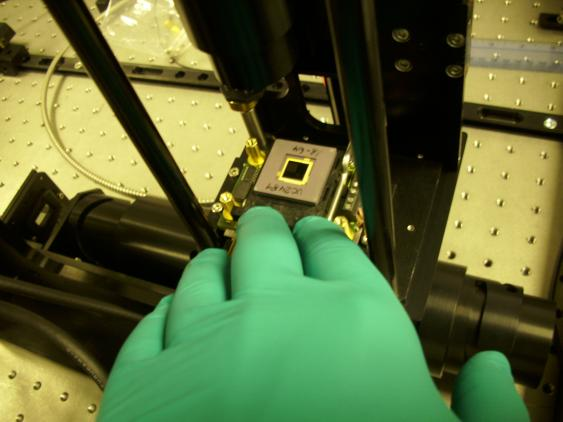
\includegraphics[width=7cm]{mma-plain}
  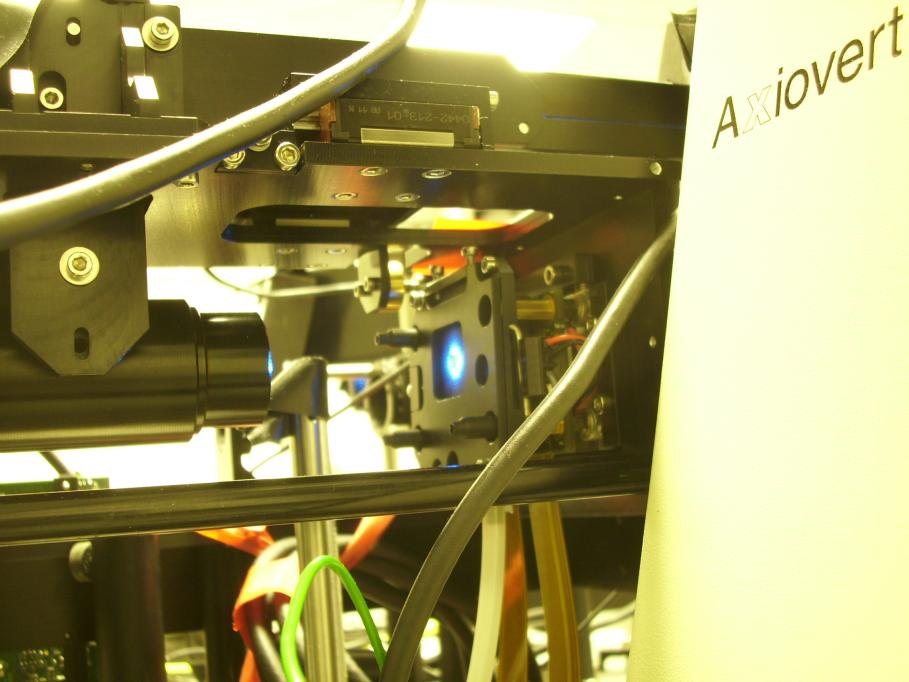
\includegraphics[width=7cm]{mma-ill}
  \caption{{\bf left:} Micro mirror array chip during installation of
    the optics. {\bf right:}~Illuminated micro mirror array in the
    aligned system.}
  \label{fig:mma-closeup}
\end{figure}

\begin{figure}[!hbt]
  \centering
  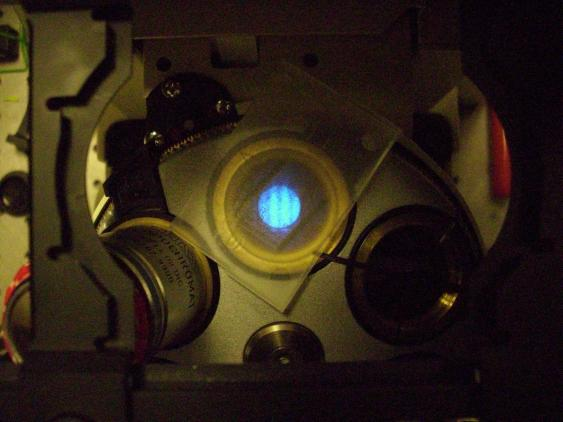
\includegraphics[width=7cm]{bfp1}
  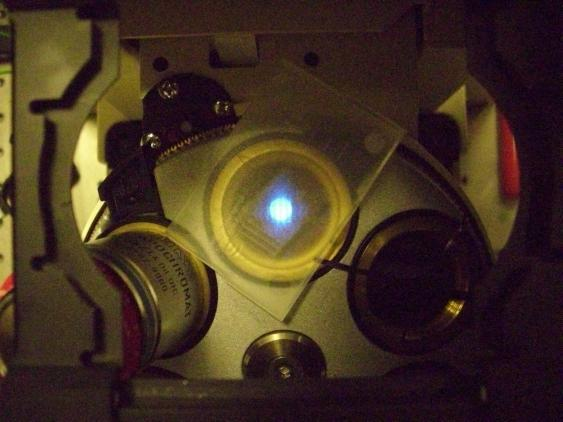
\includegraphics[width=7cm]{bfp2}
  \caption{Images of the micro mirror array in the back focal plane
    with different settings of the variable tube lens. The micro mirror
    array displays the same image (a disk) in both cases.}
  \label{fig:tubelens-bfp}
\end{figure}

\imagw{5cm}{lcos}{The black cylinder on the left is the variable tube
  lens. Behind this is the polarizing beam splitter and the
  ferroelectric liquid crystal on silicon display.}
\newpage
\section{Electronics for synchronization}
Both spatial light modulators can run at most with $50\%$ duty
cycle. Therefore it is necessary to synchronize the displays. Their
controllers allow to upload several hundred frames of image data
before an experiment and keep them in local storage. Images can then
be selected by fast function calls over USB (LCoS) or Ethernet (MMA).

The camera (Andor Clara) as the slowest device is chosen as the
master. The camera provides two TTL outputs. The output ``fire'' is
high while the camera is integrating. The output ``shutter'' goes high
\unit[1]{ms} before ``fire'' and provides enough time
(\unit[$>850$]{$\mu$s}) for the MMA controller to tilt and let the
mirrors settle.

The LCoS controller can only be programmed to a limited number of
discrete image times (\unit[20]{ms}, \unit[10]{ms}, \unit[5]{ms},
\unit[200]{$\mu$s}) and it is not straight forward to change this via
USB interface. Therefore we always work with a fixed integration time
of \unit[20]{ms}. The ``fire'' output of the camera also switches the
laser on using an acousto-optic modulator (AOM).

When the z-stage is used, the camera is stopped until the stage has
reached its target position.

\begin{figure}[!hbt]
  \centering
  \input{memi-electronics.eps_tex}
  \caption{The camera triggers both spatial light modulators with its
    TTL outputs. The acousto-optic modulator sends light into the
    system during camera integration.}
  \label{fig:memi-electronics}
\end{figure}

\section{Alignment of the displays}

In order to be able to predict which position on the camera will be
illuminated by a particular pixel of the LCoS a calibration procedure
is run. For this a fluorescent plane is selected as a specimen. Then
single spots are scanned for a grid of $10\times10$ positions over the
LCoS. The resulting spots on the camera are located and four
parameters defining the rigid transform between camera and LCoS are
estimated (scale, rotation angle, translation in x and y, see
Appendix~\ref{sec:rigid}).

Using these parameters one can then convert between camera and LCoS
coordinates (see \figref{fig:screen_lcos-calib}). Changing the focal
length of the illumination tube lens or a change on the camera position
generally requires a new calibration.

\imagw{7cm}{screen_lcos-calib}{{\bf left:} Mask that is displayed on
  the LCoS. {\bf right:} Camera image of fluorescent plane illuminated
  by mask. The orange lines indicate the borders of the original
  pattern.}

The MMA is aligned by displaying an annular ring on the MMA and
matching it to the ring of a phase objective.


\section{Ray-based illumination optimization}
In order to make use of the spatio-angular illumination system it is
necessary to produce masks for the two spatial light modulators, that
will reduce unnecessary illumination in the sample.

\subsection{Index matched sphere model}
\label{sec:shadow-map}
One useful simple model are spheres. They can model fluorescent beads
or nuclei in a \emph{C.~elegans} embryo. \figref{fig:render} displays
a model of a \emph{C.~elegans} embryo, constructed from
three-dimensional data of a confocal microscope. The nuclei are
relatively sparse. In order to illuminate one or a few nuclei we might
be able to find a path for the excitation light that doesn't intersect
out-of-focus nuclei -- or at least avoids them. In our spatio-angular
microscope the illumination pattern is represented by two masks. One
for the LCoS and another one for the MMA. In the following we will
construct an algorithm to find such optimized illumination
patterns. For example the red rectangle (with $\sim\unit[4]{\mu m}$ on
the side) would be selected for illumination with the LCoS. The red
cylinder indicates the angle that would be least obscured by
out-of-focus nuclei.

\imagw{6cm}{render}{Rendering of a sphere model, fitted to one time
  frame of a three-dimensional confocal video of a developing
  \emph{C. elegans} embryo (strain AZ212, data provided by Jean-Yves
  Tinevez (Institut Pasteur, Paris) by finding local maxima in the
  difference of Gaussian filtered data \citep{Santella2010}.}

\subsection{Tracing in illumination direction}
\imagw{12cm}{scan-mosaic_testsample_n100_3_7_5_big_label}{Test case
  for spatio-angular illumination. A target sphere is moved out of a
  layer of spheres. {\bf (a-c)} Rays from the back focal plane are
  traced through the target sphere and the total intersection length
  with out-of-focus spheres is plotted in the diagrams.}

First we assume the beads are embedded in index matched medium. Then
rays only refract at the Gaussian sphere of the objective lens and it
is insignificant how far the target bead is from the interface between
coverslip and medium.

Initially we investigated a very simple optimization routine (see
\figref{fig:scan-mosaic_testsample_n100_3_7_5_big_label}). A circular
window with radius $r$ is placed into the back focal plane. Rays from
the centre and periphery of the window are traced through the target
and into out-of-focus spheres. The intersection length of each ray
with each sphere is summed and plotted into a diagram.

\figref{fig:scan-mosaic_testsample_n100_3_7_5_big_label}~a) depicts
the collected values for a point-like window.
\figref{fig:scan-mosaic_testsample_n100_3_7_5_big_label}~b) shows the
same for a window with a diameter of 5\% of the back focal plane. The
left column in the table below the images lists the minimal values
over the full back focal plane. For small windows, a few of the rays
can hit the target without intersecting any other spheres. Increasing
the window size blurs the features in the diagrams.

Here we would choose the window with $r=0.15$
(\figref{fig:scan-mosaic_testsample_n100_3_7_5_big_label}~c)). It
still has a low minimum but the largest amount of light would reach
the target.

\imagw{12cm}{scan-mosaic_nuc12_n100_3_7_5_big_label}{Raytrace for
  circular window optimization in illumination direction. A window
  with 33\% BFP diameter would be used to illuminate the target
  nucleus.}

\figref{fig:scan-mosaic_nuc12_n100_3_7_5_big_label} shows a similar
raytrace for a sphere model of a \emph{C.~elegans} embryo and chooses
a window size and position which in this sense is optimal.

However with the MMA we have a very versatile display and we don't
have to limit ourselves to circular windows. Also the raytraced
optimizations can look noisy when not enough rays are sent through the
sample.
\subsection{Tracing in detection direction}
\label{sec:trace-detect}
For this reason we decided to trace rays from out-of-focus nuclei
through the target into the back focal plane.

\figref{fig:img2-montage_hor}~C) depicts the results of tracing
through a single target point and the out-of-focus spheres in B) in
illumination direction. Note how each out-of-focus spheres result in a
deformed blob in the back focal plane. 

It should be quite clear that the image in
\figref{fig:img2-montage_hor}~D) displays nearly the same information
but was obtained with much less computation.  Here 16 rays were trace
(see Appendix~\ref{sec:sphere-projection}) from the periphery of each
out-of-focus nucleus and one from the centre and the resulting
triangle fan was rasterized into the image. We call this image a
shadow map.


In order for our spatio-angular system to work, neither the MMA, nor
the LCoS should displays masks with only a few white pixels. Ray based
simulations are not good models in this case (see
Appendix~\ref{sec:sim-angle} for a description of a wave optical
treatment) and illumination light would simply be impractically low.

For this reason the trace of \figref{fig:img2-montage_hor}~D) is
insufficient. Instead of one target point a sufficiently big area in
the model should be sampled. We sum each of the corresponding shadow
maps into a new one (see the two images on the left in
\figref{fig:bfp2-bfp-images-and-model}. Then we threshold the
accumulated shadow map, so that only the angles with least
out-of-focus targets are illuminated. Finally we blur the mask with a
Gaussian filter in order to prevent ringing in sample space.

The diagram on the right of \figref{fig:bfp2-bfp-images-and-model}
displays a sphere model of three-dimensionally distributed beads
($\unit[2]{\mu m}$ diameter, yellow-green, in oil). We obtained this
model with our microscope by displaying several gratings on the LCoS
at full angular illumination and doing a structured illumination
reconstruction (in each pixel the maximum of each pattern minus minimum
of each pattern) of sectioned slices. A matching difference of
Gaussian filter and local maximum search in the three-dimensional
volume gives the centres of the beads.

After constructing the model, the microscope continuously moves the
z-stage onto each bead and illuminates them with their optimized
illumination angles. Bead~26 has been illuminated with very high
angles in order to prevent exposure of the bunch of beads further away
from the objective. Bead~5 is far from any other beads and therefore
more angles can be used for its illumination.


\imagw{14cm}{img2-montage_hor}{{\bf A)} Schematic of the rays between
  back focal plane and sample. {\bf B)} Out-of-focus spheres and the
  target point define a double cone of rays that should not be
  illuminated. {\bf C)} Tracing rays in illumination direction from
  the back focal plane through the sample is an expensive operation
  and results in unnecessarily exact results. {\bf D)} Tracing in
  detection direction from the periphery of out-of-focus spheres
  through a target point into the back focal plane gives nearly
  identical results (shadow map) and is more computationally
  efficient.}

% some raw data with beads in dvi system:
% /mnt/backup/backups-london/mnt/floh/sda3/martin/0226/winterseminar/0216_6
\imagw{10cm}{bfp2-bfp-images-and-model}{{\bf right:} Sphere model of a
  sample with three-dimensionally distributed beads. {\bf left:}
  Optimized MMA masks to illuminate bead 26 or bead 5. The red circles
  indicate the periphery of the BFP of the objective.}



%\imagw{12cm}{structured}{Images of a $\unit[3]{\mu m}$ bead within
%  slightly fluorescent embedding medium under different illumination
%  conditions using a $63\times/1.38$ objective.}




\subsection{Coping with index mismatch of the embedding medium}
So far the described algorithms assumed ideal samples which have been
embedded in a medium with a refractive index, the objective was
designed for.

Biological samples are often embedded in water. However, it might
still be useful, to image with an oil objective. Then the additional
refraction at the glass--water interface has to be taken into account
for spatio-angular illumination.

This makes the task of predicting where to mask the MMA in order to
protect out-of-focus beads more complicated. To circumvent the
spherical aberrations, we have to limit the range of angles, that are
simultaneously illuminating and shift the illumination spot on the
LCoS to correct for the transversal focus shift ($q$ in
\figref{fig:aberration-sketch} right). For this we must have a good
estimate of the distance of the sample from the coverslip--water
interface. See Appendix~\ref{sec:raytrace} for a description of the
raytrace algorithm.

Using an oil immersion objective has the following advantage: By
sending the illumination rays into the sample at a steep angle, close
to the TIRF angle, we can generate a thin sheet of light (see
\figref{fig:hilo}).


\begin{figure}[!hbt]
  \centering
  \def\svgscale{.3}
  \input{screen_0_lines.eps_tex}\qquad
  \input{aberration-sketch.eps_tex}
  \caption{{\bf left:} Rays are starting from periphery of
    out-of-focus nucleus, hitting the target and refracted at the
    water--coverslip interface. {\bf right:} Due to spherical
    aberrations, rays from an on-axis point are shifted to $q(r)$ on
    the camera (where $r$ relates to the angle of the ray in the
    sample). }
  \label{fig:aberration-sketch}
\end{figure}

\begin{figure}[!hbt]
  \centering
  \def\svgscale{.3}
  \input{shift-correction.eps_tex}
  \caption{{\bf top:} A straight ray illuminates a bead embedded in
    oil. {\bf middle:} Embedding the sample in water results in
    refraction of the ray. {\bf bottom:} The refraction can be
    compensated by shifting the target area on the LCoS.}
  \label{fig:shift-correction}
\end{figure}
 
% our reports: they were often corrected by Susan, so i should have a look
% MEMI_WP6_D6_5_Report.pdf     angular clem with grating on lcos
% 6.7    drawing of setup, alignment, sync image, only 11 of the 24 bitplanes
% 6.8a   full field angular control with mma (i used too large images on lcos)
%        rendering of c. elegans embryo, psf calc, ray model,
%        first (yellow) raytraces
% 8.6a   sync image with 11 out of 24
